\documentclass[border=10pt]{standalone}

\usepackage{tikz}
\usepackage{tikzsymbols}
\usetikzlibrary{calc,patterns,shapes.geometric}

\def\centerarc[#1](#2)(#3:#4:#5){\draw[#1] ($(#2)+({#5*cos(#3)},{#5*sin(#3)})$) arc (#3:#4:#5);}

\begin{document}
	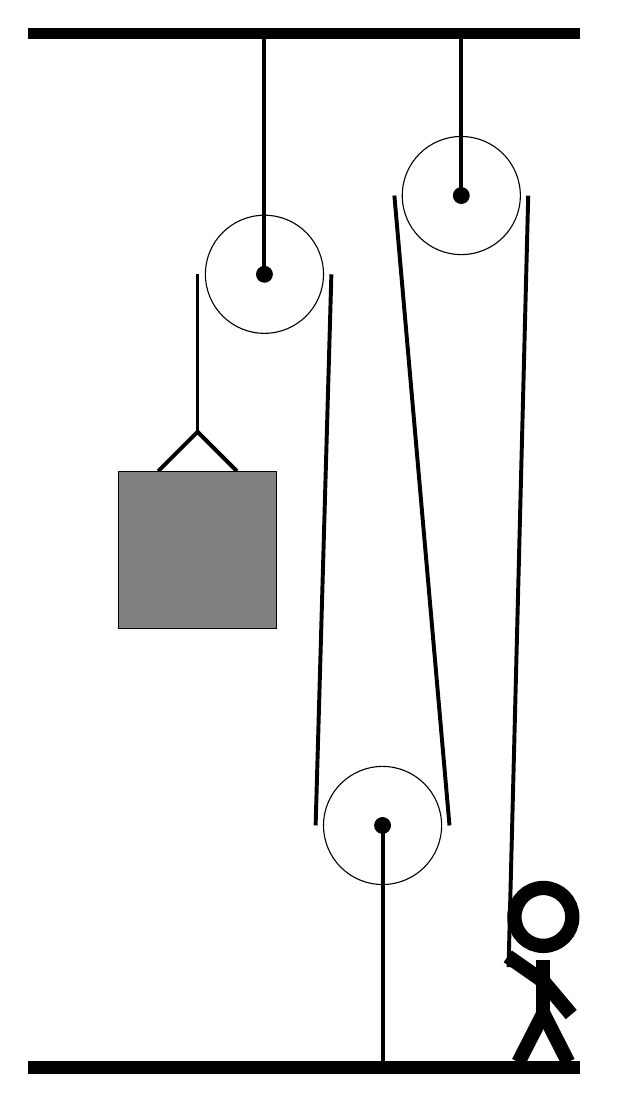
\begin{tikzpicture}
		%%%%% START %%%%%
		\draw[fill=black] (-2, 10) rectangle (5, 10.125);
		
		\draw (1, 7) circle (0.75);
		\draw[fill=black] (1, 7) circle (0.1);
		\draw[line width=0.5mm]  (1, 10) -- (1, 7);
		
		\draw[fill=white](2.5, 0) circle (0.75);
		\draw[fill=black] (2.5, 0) circle (0.1);
		\draw[line width=0.5mm]  (2.5, -3) -- (2.5, 0);
		
		\draw[fill=white](3.5, 8.0) circle (0.75);
		\draw[fill=black] (3.5, 8.0) circle (0.1);
		\draw[line width=0.5mm] (3.5, 10) -- (3.5, 8.0);
		
		\draw[line width=0.5mm] (-0.35, 4.5) -- (0.15, 5.0) -- (0.65, 4.5);
		\draw[fill=black!50] (-0.85, 4.5) rectangle (1.15, 2.5);
		
		\draw[line width=0.5mm] (0.15, 7) -- (0.15, 5.0);
		\centerarc[line width=0.5mm](1, 7)(0:180:0.85);
		\draw[line width=0.5mm](1.85, 7) -- (1.65, 0);
		\centerarc[line width=0.5mm](2.5, 0)(180:360:0.85);
		\draw[line width=0.5mm](3.35, 0) -- (2.65, 8.0);
		\centerarc[line width=0.5mm](3.5, 8.0)(0:180:0.85);
		\draw[line width=0.5mm](4.35, 8.0) -- (4.1, -1.8);
		
		\node at (4.5, -1.9) {\Strichmaxerl[10][-35][-50]};
		
		\draw[fill=black] (-2, -3) rectangle (5, -3.15);
		%%%%% END %%%%%
	\end{tikzpicture}
\end{document}